% \documentclass[aspectratio=169,notes]{beamer}
\documentclass[aspectratio=169]{beamer}
\usetheme[faculty=phil]{fibeamer}
\usepackage{polyglossia}
\setmainlanguage{english} %% main locale instead of `english`, you
%% can typeset the presentation in either Czech or Slovak,
%% respectively.
\setotherlanguages{russian} %% The additional keys allow
%%
%%   \begin{otherlanguage}{czech}   ... \end{otherlanguage}
%%   \begin{otherlanguage}{slovak}  ... \end{otherlanguage}
%%
%% These macros specify information about the presentation
\title[AGLA1]{Analytical Geometry and Linear Algebra I, Lab 5} %% that will be typeset on the
\subtitle{Test 1 Solutions \\ Matrix Rank \\ Q/A session   
         } %% title page.
\author{Oleg Bulichev}
%% These additional packages are used within the document:
\usepackage{ragged2e}  % `\justifying` text
\usepackage{booktabs}  % Tables
\usepackage{tabularx}
\usepackage{tikz}      % Diagrams
\usetikzlibrary{calc, shapes, backgrounds}
\usepackage{amsmath, amssymb}
\usepackage{url}       % `\url`s
\usepackage{listings}  % Code listings
% \usepackage{subfigure}
\usepackage{floatrow}
\usepackage{subcaption}
\usepackage{mathtools}
\usepackage{todonotes}
\usepackage{fontspec}
\usepackage{multicol}
\usepackage{pdfpages}
\usepackage{wrapfig}
\usepackage{animate}
\usepackage{booktabs}
\usepackage{multirow}

\graphicspath{{resources/}}
\frenchspacing

\setbeamertemplate{caption}[numbered]
\usetikzlibrary{graphs}

% \usepackage[backend=biber,style=ieee,autocite=footnote]{biblatex}
% \addbibresource{biblio.bib}
% \DefineBibliographyStrings{english}{%
%   bibliography = {References},}

\newcommand{\oleg}[2][] {\todo[color=red, #1] {OLEG:\\ #2}}
\newcommand{\fbckg}[1]{\usebackgroundtemplate{\includegraphics[width=\paperwidth]{#1}}}%frame background

\usepackage[framemethod=TikZ]{mdframed}
\newcommand{\dbox}[1]{
\begin{mdframed}[roundcorner=3pt, backgroundcolor=yellow, linewidth=0]
\vspace{1mm}
{#1}
\vspace{1mm}
\end{mdframed}
}

\begin{document}
\setlength{\abovedisplayskip}{0pt}
\setlength{\belowdisplayskip}{0pt}
\setlength{\abovedisplayshortskip}{0pt}
\setlength{\belowdisplayshortskip}{0pt}

\fbckg{fibeamer/figs/title_page.png}
\frame[c]{\setcounter{framenumber}{0}
    \usebeamerfont{title}%
    \usebeamercolor[fg]{title}%
    \begin{minipage}[b][6.5\baselineskip][b]{\textwidth}%
        \textcolor{black}{\raggedright\inserttitle}
    \end{minipage}
    % \vskip-1.5\baselineskip

    \usebeamerfont{subtitle}%
    \usebeamercolor[fg]{framesubtitle}%
    \begin{minipage}[b][3\baselineskip][b]{\textwidth}
        \raggedright%
        \insertsubtitle%
    \end{minipage}
    \vskip.25\baselineskip
}
%   \frame[c]{\maketitle}
\note{
    \begin{enumerate}
        \item Чилл пара

    \end{enumerate}
}

\fbckg{fibeamer/figs/common.png}


\begin{frame}[c]{Questions from the class}
\framesubtitle{}
\centering
    \textit{ \Large No questions for today}
\end{frame}


\begin{frame}[t]{Test 1, Solutions}
\framesubtitle{Task 1}
(2 points) Decompose the vector $\textbf{p} = (1, 2, 3)$ into components parallel and perpendicular to the vector $\textbf{q} = (1, -2, 2)$.
\end{frame}

\begin{frame}[t]{Projection}
    \framesubtitle{Definition}
    \vspace{-0.3cm}
    \begin{columns}[T,onlytextwidth]
        \begin{column}{0.5\textwidth}
            The \textit{vector projection} of a vector $\mathbf {a}$ on (or onto) a nonzero vector $\mathbf {b}$, sometimes denoted $\operatorname {proj} _{\mathbf {b} }\mathbf {a}$  is the orthogonal projection of $\mathbf {a}$ onto a straight line parallel to $\mathbf {b}$.
        \end{column}
        \begin{column}{0.49\textwidth}
            \vspace{-1cm}
            \begin{figure}[H]
                \centering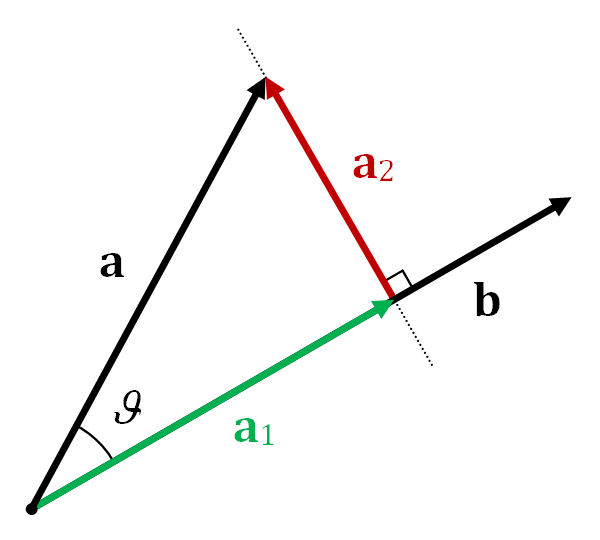
\includegraphics[height=3cm,width=1\textwidth,keepaspectratio]{Projection_and_rejection.png}
                \caption*{Projection of $\mathbf{a}$ on $\mathbf{b}$ ($\mathbf{a}_1$), and rejection of $\mathbf{a}$ from $\mathbf{b}$ ($\mathbf{a}_2$)}
                \label{fig:Projection_and_rejection.png}
            \end{figure}
        \end{column}
    \end{columns}
    \textbf{Where it can be used:}
    \vspace{-0.5cm}
    \begin{multicols}{2}
        \begin{itemize}
            \item Maps
            \item Blueprints
            \item Fitting algorithms (Least squares)
            \item Reduce matrix dimension
            \item Reinforcement Learning (RL) fitness functions
        \end{itemize}
    \end{multicols}
\end{frame}

\begin{frame}[t]{Projection}
    \framesubtitle{2D Case, Classical way \\ Project $\vec{b}$ on $\vec{a}_1$}
    \vspace{-0.8cm}
    \begin{columns}[T,onlytextwidth]
        \begin{column}{0.49\textwidth}
            \begin{align*}
                e = b -a_1x,\ \text{ $e$ --- error b/w similar vectors} \\
                a_1 \cdot (b-a_1x)=0 \\
                a_1^T(b-a_1x)=0 \\
                a_1^Tb = a_1^Ta_1x \\
                \dfrac{a_1^Tb}{a_1^Ta_1} = x \text{ --- Classical formula from school}
                \end{align*}
        \end{column}
        \begin{column}{0.49\textwidth}
            \vspace{-1.8cm}
            \begin{figure}[H]
                \centering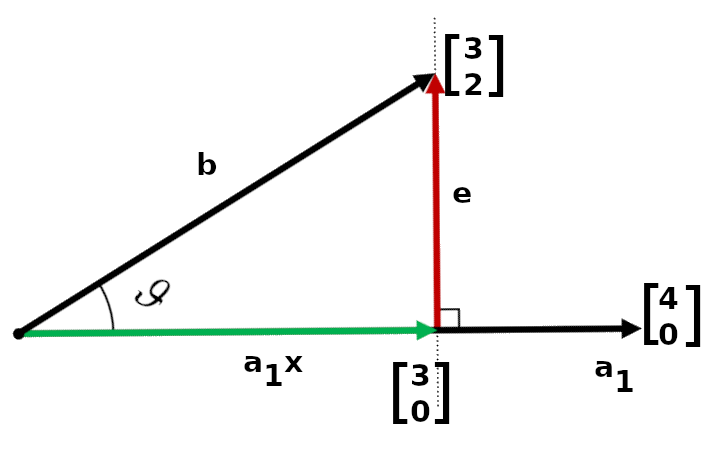
\includegraphics[height=3cm,width=1\textwidth,keepaspectratio]{resources/fig1.png}
                \label{fig:resources/fig1.png}
            \end{figure}
            \vspace{-1cm}
            \textbf{Case study}
            \begin{align*}
            \dfrac{a_1^Tb}{a_1^Ta_1} = x \Rightarrow
            \dfrac{\begin{bmatrix}4&0\end{bmatrix}\begin{bmatrix}3\\2\end{bmatrix}}{\begin{bmatrix}4&0\end{bmatrix}\begin{bmatrix}4\\0\end{bmatrix}}=\dfrac{3}{4} \\
            \text{Projection } p=a_1x = \dfrac{3}{4} \begin{bmatrix}4\\0\end{bmatrix} = \begin{bmatrix}3\\0\end{bmatrix}
            \end{align*}
        \end{column}
    \end{columns}
\end{frame}
\begin{frame}[t]{Projection}
    \framesubtitle{2D Case, Projection matrix \\ \ }
    \vspace{-0.8cm}
    \begin{columns}[T,onlytextwidth]
        \begin{column}{0.49\textwidth}
            \begin{align*}
                \left.\begin{matrix}
                Pb = xa_1 = a_1x \\
                \dfrac{a_1^Tb}{a_1^Ta_1} = x \\
                \end{matrix} \right\} P = \dfrac{a_1a_1^T}{a_1^Ta_1}
                \end{align*}
                Where $P$ --- projection matrix
        \end{column}
        \begin{column}{0.49\textwidth}
            \vspace{-1.8cm}
            \begin{figure}[H]
                \centering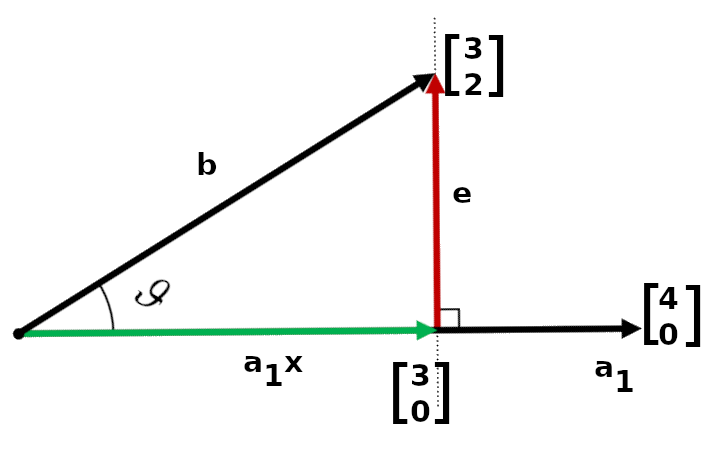
\includegraphics[height=3cm,width=1\textwidth,keepaspectratio]{resources/fig1.png}
                \label{fig:resources/fig1.png}
            \end{figure}
            \vspace{-1cm}
            \textbf{Case study}
            \begin{align*}
                P = \dfrac{a_1a_1^T}{a_1^Ta_1} = \dfrac{\begin{bmatrix}4\\0\end{bmatrix}\begin{bmatrix}4&0\end{bmatrix}}{\begin{bmatrix}4&0\end{bmatrix}\begin{bmatrix}4\\0\end{bmatrix}} = \begin{bmatrix}1&0\\0&0\end{bmatrix}\\
                p = Pb = \begin{bmatrix}1&0\\0&0\end{bmatrix}\begin{bmatrix}3\\2\end{bmatrix} = \begin{bmatrix}3\\0\end{bmatrix}
                \end{align*}
        \end{column}
    \end{columns}
\end{frame}

\begin{frame}[t]{Projection}
    \framesubtitle{2D Case, Projection matrix \\ Project $\vec{b}$ on $\vec{a}_2$, which is perpendicular to $\vec{a}_1$ }
    \vspace{-0.4cm}
    \begin{columns}[T,onlytextwidth]
        \begin{column}{0.49\textwidth}
            \begin{align*}
                P_{d_1} = I - P = \begin{bmatrix}0&0\\0&1\end{bmatrix}
                \end{align*}
                Where $P=\begin{bmatrix}1&0\\0&0\end{bmatrix}$
                
                $P_{d_1}$ is an error between the whole space and current projection matrix.
                
                $p_{d_1} = P_{d_1}b = \begin{bmatrix}0\\2\end{bmatrix}$
        \end{column}
        \begin{column}{0.49\textwidth}
            \begin{figure}[H]
                \centering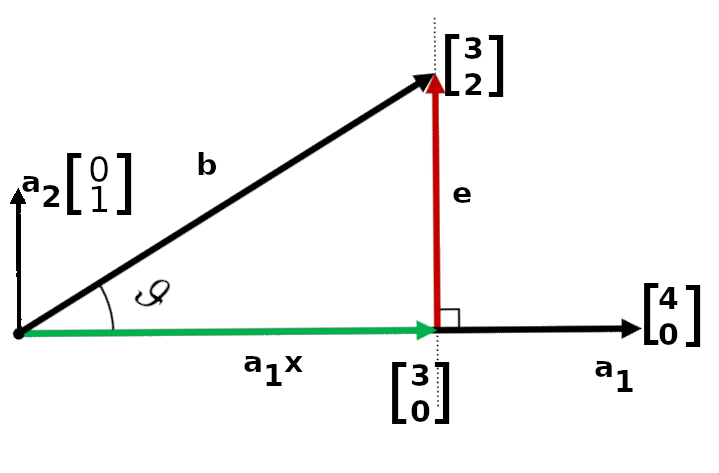
\includegraphics[height=3cm,width=1\textwidth,keepaspectratio]{resources/fig2.png}
                \label{fig:resources/fig2.png}
            \end{figure}

        \end{column}
    \end{columns}
\end{frame}

\begin{frame}[t]{Projection}
    \framesubtitle{Case study: Reinforcement Learning fitness function}
    \vspace{-0.75cm}
    \begin{columns}[T,onlytextwidth]
        \begin{column}{0.49\textwidth}
            \begin{block}{Goal}
                It is necessary for the robot to move in a straight line in all directions, as well as as as efficiently as possible. 
                
                The efficiency criteria are: course deviation error, max velocity and clearance.
            \end{block}
            \vspace{-0.5cm}
            \begin{flalign*}
                F = \omega_1X_z + \omega_2\frac{1}{|err| + \varepsilon}+ \omega_3(P_{d_{real}}\vec{X})\text{, where} \\
                err = |(I-P_{d_{real}})(I-P_{n_{pl}})\vec{X}|,\\
                \text{$P_{*}$ -- projection matrix, $\omega_{*}$ -- weight coeffs.}
            \end{flalign*}
        \end{column}
        \begin{column}{0.49\textwidth}
            \begin{figure}[H]
                \centering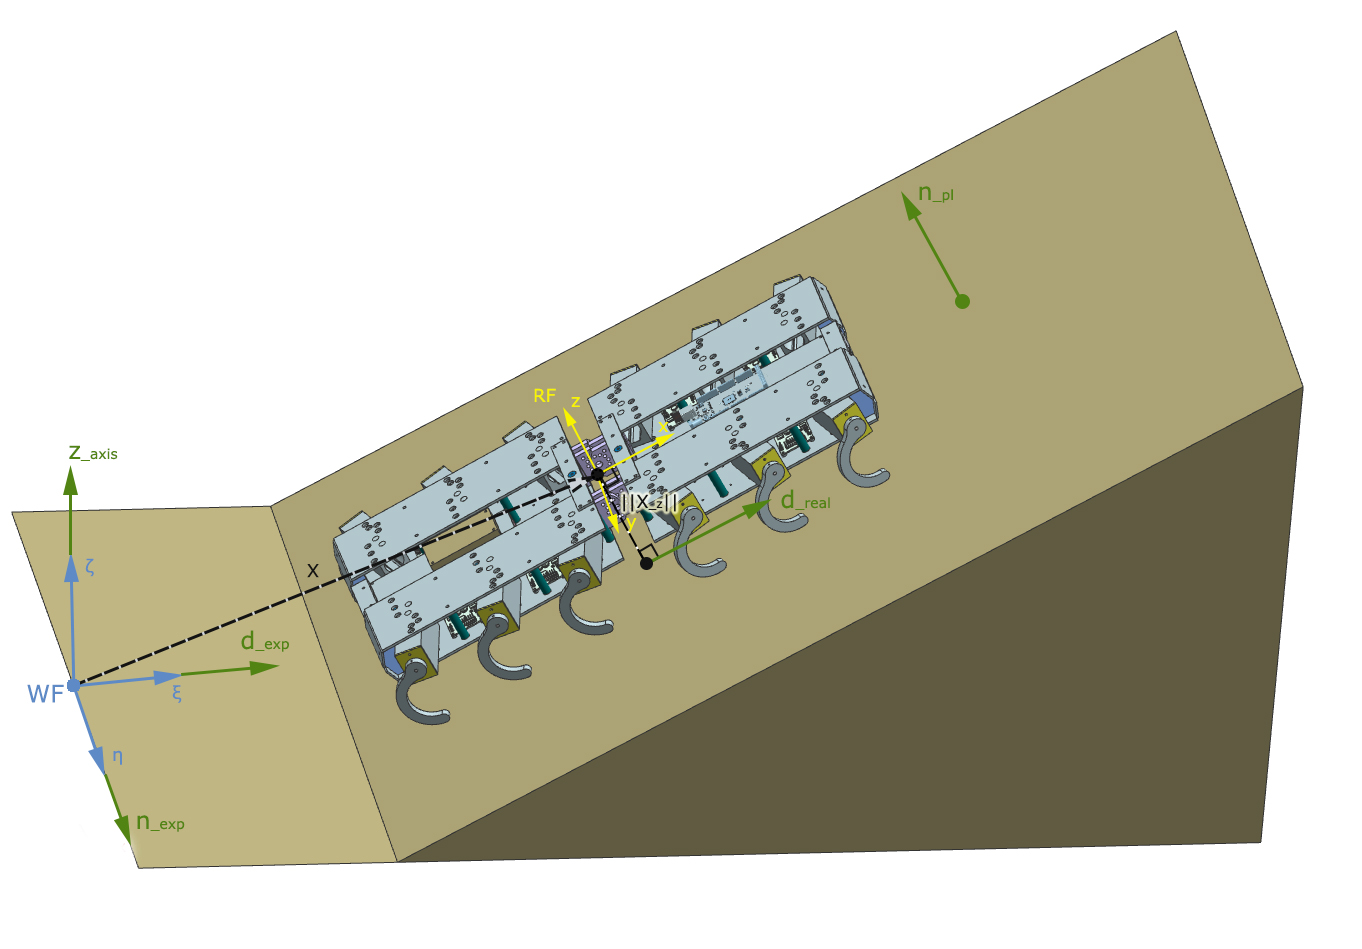
\includegraphics[height=6cm,width=1\textwidth,keepaspectratio]{strirus_full_body_on_plane_first.jpg}
                \caption*{\large StriRus -- task description}
                \label{fig:strirus_full_body_on_plane_first.jpg}
            \end{figure}
        \end{column}
    \end{columns}
\end{frame}

\begin{frame}[t]{Task 1}
    \framesubtitle{Answer}
        \begin{figure}[H]
            \centering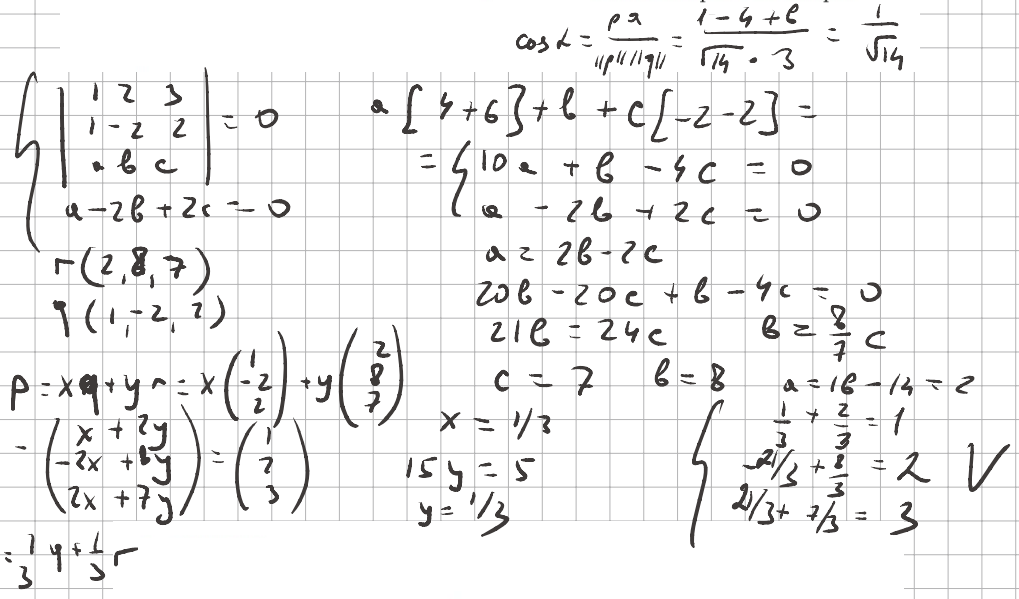
\includegraphics[height=5.5cm,width=1\textwidth,keepaspectratio]{1ans.png}
            % \caption{caption_name}
            \label{fig:1ans.png}
        \end{figure}
\end{frame}

\begin{frame}[t]{Task 2}
    \framesubtitle{}
    \only<1>{
        \begin{enumerate}
            \item Find the matrix product $AB$ if $A=\begin{bmatrix}x & -2 & -1 \\ 4 & 1 & -4 \end{bmatrix}$, $B=\begin{bmatrix} -5 & 1 \\ 1 & -3 \\ 2 & x \end{bmatrix}$
            \item Find the largest possible value of determinant $(AB)$.
        \end{enumerate}}
    \only<2>{
        \alert{\Large Answer}
        \begin{figure}[H]
            \centering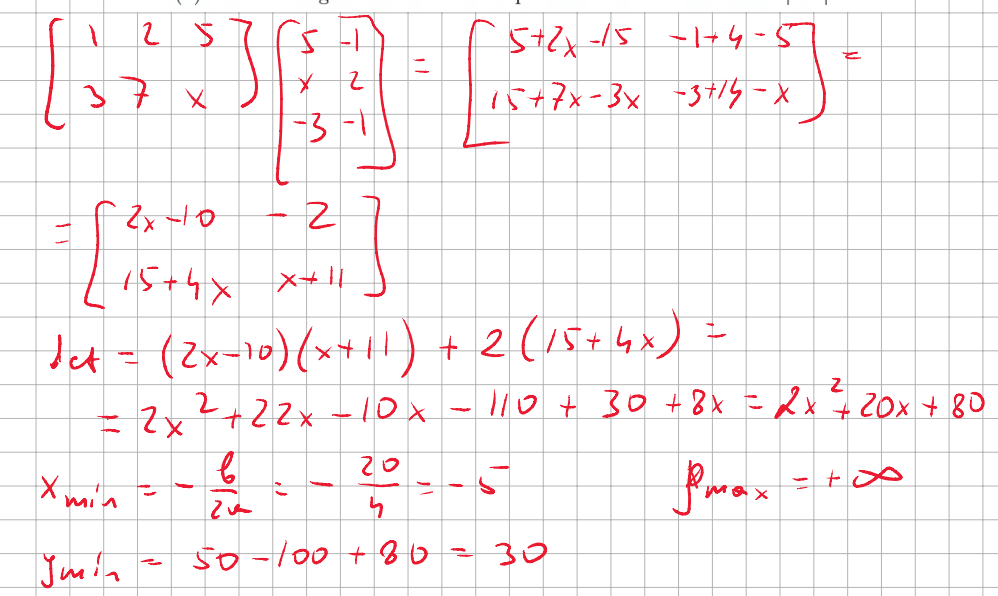
\includegraphics[height=5.5cm,width=1\textwidth,keepaspectratio]{2ans.png}
            % \caption{caption_name}
            \label{fig:2ans.png}
        \end{figure}
    }
\end{frame}

\begin{frame}[t]{Task 3}
    \framesubtitle{}
    \only<1>{
        For which values $x$, vectors \textbf{a} and \textbf{b} are basis of some space? Explain your answer. \\
        $\textbf{a} =  \begin{bmatrix} 1-x \\ x  \end{bmatrix}$,
        $\textbf{b} =  \begin{bmatrix} 1-x \\ -2     \end{bmatrix}$}
    \only<2>{
        \alert{\Large Answer}
        \begin{figure}[H]
            \centering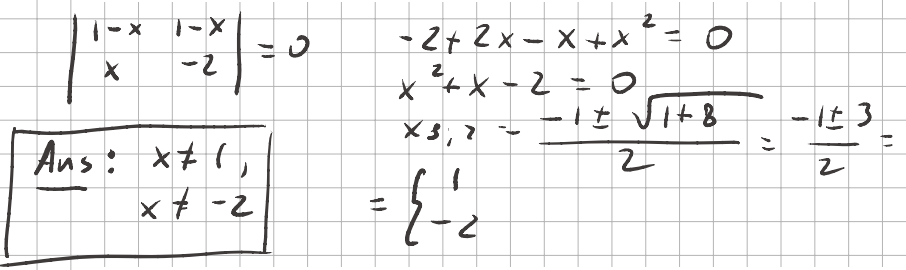
\includegraphics[height=5.5cm,width=1\textwidth,keepaspectratio]{3ans.png}
            % \caption{caption_name}
            \label{fig:3ans.png}
        \end{figure}
    }
\end{frame}

\begin{frame}[t]{Task 4}
    \framesubtitle{}
    \only<1>{
        Given a parallelogram $ABCD$. Point $N$ is the crossing of its diagonals. The old coordinate system has origin $A$ and the basis  $AB$, $AD$.

        \begin{enumerate}
            \item Define a new coordinate system formed by the point $D$ and two new basis vectors: $DB$ and $DC$. 
            \item Compute the transitions matrix $A$ from the old basis to the new basis.
            \item Calculate coordinates of point $N$ in both bases, using the transition matrix $A$.
        \end{enumerate}}
    \only<2>{
        \alert{\Large Answer}
        \begin{figure}[H]
            \centering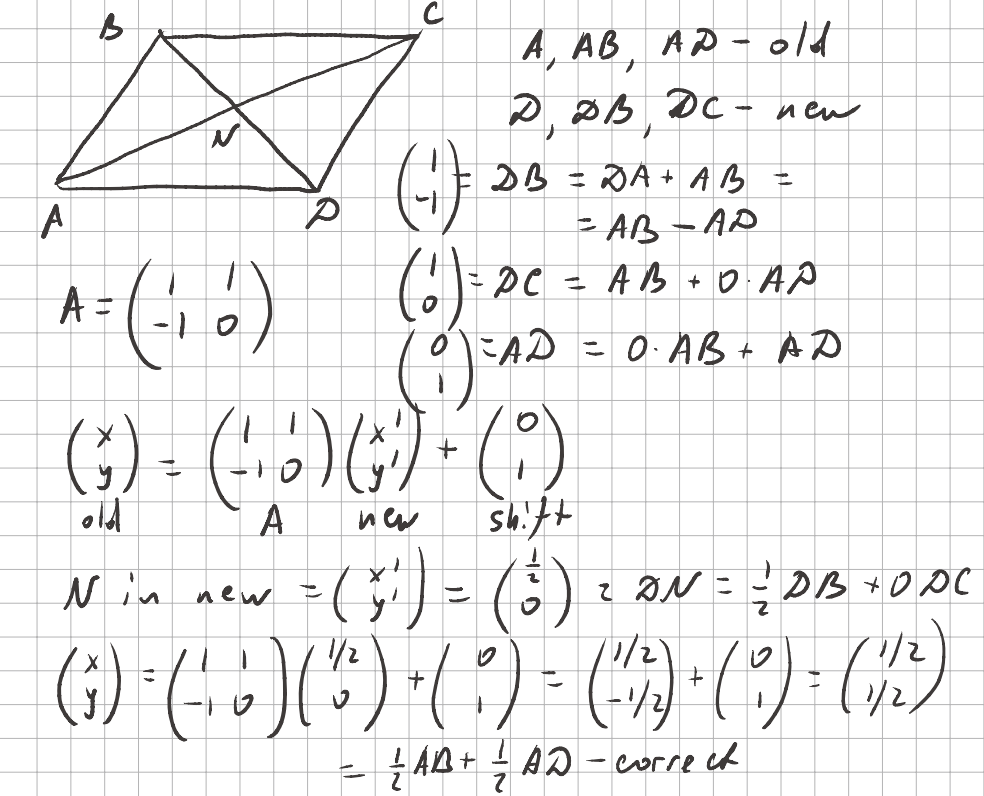
\includegraphics[height=5.5cm,width=1\textwidth,keepaspectratio]{4ans.png}
            % \caption{caption_name}
            \label{fig:4ans.png}
        \end{figure}
    }
\end{frame}

\begin{frame}[t]{How to get out of an exam}
    \framesubtitle{Video}
    \vspace{-0.6cm}
    \begin{figure}[H]
        \href{https://youtu.be/eiLF4zRA634}{
            \centering
\includegraphics[height=6cm,width=1\textwidth,keepaspectratio]{meme.jpg}}
        % \caption{Click on a picture for a video}
        \label{fig:meme.jpg}
    \end{figure}
\end{frame}

\begin{frame}[t]{Matrix Rank}
    \framesubtitle{Definition}
        \textbf{$N_r(A)$} --- max number of \textbf{lineary independent} rows of matrix $A$.
    
        \textbf{$N_c(A)$} --- max number of \textbf{lineary independent} columns of matrix $A$.
    
        \begin{equation*}
            Rank(A) = N_r(A) = N_c(A)
        \end{equation*}
    \bigskip
    
        \centering
        The rank of the matrix is how many of the rows (columns) are <<unique>>: not formed out by other rows (columns).
    \end{frame}
    
    \begin{frame}[t]{Matrix Rank}
    \framesubtitle{Motivation}
        \begin{itemize}
            \item Computation of the number of solutions of a system of linear equations.
            \item Analysis of the linear dependency of rows and columns.
            \item Applications in Control Theory (next year): observability and controllability.
        \end{itemize}
    \end{frame}
    
    \begin{frame}[t]{Matrix Rank}
    \framesubtitle{How to find}
        There are 3 ways:
        \begin{enumerate}
            \item \textbf{Look at matrix} and find linear dependencies.
            \item \textbf{Reduced form} (transform matrix to upper triangular form (The first part of the algorithm for finding inverse matrix).
            \item \textbf{Minor method} (\href{http://www.mathprofi.ru/rang_matricy.html}{Метод окаймляющих миноров} ) \textit{not popular in western education}.
        \end{enumerate}
    \end{frame}


\begin{frame}[t]{Matrix Rank}
\framesubtitle{Case Study (on whiteboard)}
Calculate the rank of the following matrix: $\begin{bmatrix}1&2&3\\2&3&4\\1&1&1\end{bmatrix}$. \medskip

\alert{\Large Answer: 2}
\end{frame}

\begin{frame}[t]{Matrix Rank}
\framesubtitle{Task 2}
Determine the ranks of the following matrices for all real values of parameter $\alpha$:
\begin{enumerate}

    \item $\begin{bmatrix}1&\alpha&-1&2\\2&-1&\alpha&5\\1&10&-6&1\end{bmatrix}$;
    \item $\begin{bmatrix}1&1&1\\1&\alpha&\alpha^2\\1&\alpha^2&\alpha\end{bmatrix}$;
\end{enumerate}
\end{frame}


\begin{frame}[t]{Reference material}
    % \framesubtitle{OnlineMschool}
    \Large
    \begin{itemize}
        \item \href{https://onlinemschool.com/math/library/matrix/rank/}{Matrix Rank (OnlineMschool)}
    \end{itemize}
\end{frame}

\fbckg{fibeamer/figs/last_page.png}
\frame[plain]{}

\end{document}